% Hand-authored roadmap for the CVPR 2027 research package.
% Compile from cvpr2027/:  .tools/tectonic docs/latex/roadmap.tex --outdir output/pdf --keep-logs
\PassOptionsToPackage{unicode}{hyperref}
\PassOptionsToPackage{hyphens}{url}
\PassOptionsToPackage{dvipsnames,svgnames,x11names}{xcolor}
\documentclass[11pt,a4paper]{article}
\usepackage{xcolor}
\usepackage[margin=24mm]{geometry}
\usepackage{amsmath,amssymb}
\usepackage{iftex}
\usepackage{lmodern}
\usepackage{textcomp}
\usepackage{parskip}
\usepackage{longtable,booktabs,array}
\usepackage{graphicx}
\usepackage{caption}
\usepackage{enumitem}
\usepackage{float}
\usepackage{needspace}
\usepackage{tikz}
\usetikzlibrary{arrows.meta,positioning,calc}
\usepackage{hyperref}
% Shared style; used by generated, standalone LaTeX sources.
\usepackage{xcolor}
\usepackage{xurl}
\usepackage{fvextra}
\usepackage{etoolbox}
\usepackage{fancyhdr}
\usepackage{titlesec}
\definecolor{researchblue}{HTML}{173B58}
\AtBeginDocument{\hypersetup{linkcolor=researchblue,urlcolor=researchblue}}
\pagestyle{fancy}
\fancyhf{}
\fancyhead[L]{\small\sffamily SVG PATCH LAB}
\fancyhead[R]{\small\sffamily CVPR 2027 research package}
\fancyfoot[L]{\small Working documents; results and proposals distinguished}
\fancyfoot[R]{\thepage}
\setlength{\headheight}{15pt}
\setlength{\emergencystretch}{3em}
\titleformat{\section}{\Large\bfseries\color{researchblue}}{\thesection}{0.7em}{}
\titleformat{\subsection}{\large\bfseries\color{researchblue}}{\thesubsection}{0.7em}{}
\DefineVerbatimEnvironment{verbatim}{Verbatim}{breaklines=true,breakanywhere=true,fontsize=\small}
\AtBeginEnvironment{longtable}{\small\setlength{\tabcolsep}{4pt}}
\let\originaltableofcontents\tableofcontents
\renewcommand{\tableofcontents}{\originaltableofcontents\clearpage}

\captionsetup{font=small,labelfont=bf}
\setlist{nosep,leftmargin=1.4em}
\newcommand{\code}[1]{\path{#1}}
\newcommand{\degC}{\,\textdegree C}
\newcolumntype{L}[1]{>{\raggedright\arraybackslash}p{#1}}
\newcolumntype{R}[1]{>{\raggedleft\arraybackslash}p{#1}}
\newcommand{\keybox}[1]{\begin{center}\fcolorbox{researchblue}{researchblue!6}{\parbox{0.94\linewidth}{#1}}\end{center}}
\hypersetup{pdftitle={Roadmap: solver-in-the-loop SVG engineering drawings from text, images and SVG},pdfauthor={SVG Patch Lab}}

\title{\color{researchblue}\LARGE Roadmap\\[6pt]\Large Solver-in-the-loop SVG engineering drawings from text, images and existing SVG --- what to build, what to train, and in what order}
\author{SVG Patch Lab \quad\textbullet\quad CVPR 2027 research package}
\date{18 September 2026 --- for review; dates are work targets, not promises}

\begin{document}
\maketitle

\keybox{\textbf{Goal.} A system that turns a text request, a picture of a part, or an existing drawing into an SVG engineering drawing whose contours are numerically true, by putting a solver (FEM, and PINN surrogates where they earn their place) between the language model and the picture. It is evaluated on the cases where direct Astra fails, because those are the only cases where such a system can be shown to add anything.}

\keybox{\textbf{Rules that shape every phase} (from the experiment protocol). Train a model only after a measured gap beyond the rule parser, prompting and the deterministic plotter. Split by physical case and geometry family before generating variants. Count every attempted output. Keep test references, outputs and inspected failures out of training. Report negative results.}

\tableofcontents

% =====================================================================
\section{Where we start from}

Already in the package and tested: the sampled-contour evaluator (C01--C02); validated solvers --- scikit-fem P2 with Robin boundaries, finite differences on rectilinear domains, the pinned FEM-Bench bar (C07, C10) --- and a validated plane-stress stack for general polygons with holes (\code{scripts/fem_smoke.py}); the twelve-task hard-drawing harness with references, scoring, overlays and browser rendering (C14); a LoRA training and evaluation pipeline that is deterministic across three GPU sessions (C05, C11, C12); the remote batch runner on a 96~GB Blackwell workstation and the Colab A100 path; and the direct-Astra API harness with cost accounting (C13, C14).

Measured so far: direct Astra is exact on closed-form and textbook fields, wrong on unseen geometry (4.5~pp mean), marginal at strong convection and on the Kirsch tensor field, honest about its status, and correct on two ill-posed cases. The editing pilot is saturated by every method. Not yet built: the image path, a benchmark that a parser cannot solve, the semantic half of the verifier, any PINN, any human study.

% =====================================================================
\section{Target system}

\begin{figure}[H]
\centering
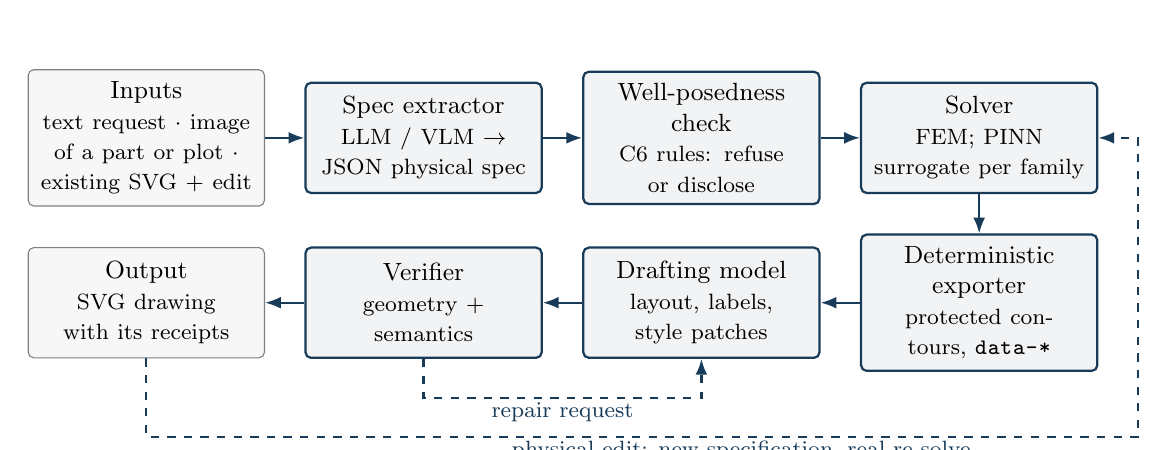
\begin{tikzpicture}[
  node distance=5mm and 5mm,
  box/.style={draw=researchblue,thick,rounded corners=2pt,fill=researchblue!6,align=center,minimum height=14mm,text width=27mm,inner sep=1.5mm,font=\small},
  src/.style={draw=black!50,rounded corners=2pt,fill=black!3,align=center,minimum height=14mm,text width=27mm,inner sep=1.5mm,font=\small},
  arr/.style={-{Latex[length=2mm]},thick,researchblue},
  lbl/.style={font=\footnotesize,fill=white,inner sep=1pt}]
  \node[src] (in) {Inputs\\\footnotesize text request $\cdot$ image of a part or plot $\cdot$ existing SVG + edit};
  \node[box,right=of in] (spec) {Spec extractor\\\footnotesize LLM / VLM $\rightarrow$ JSON physical spec};
  \node[box,right=of spec] (wp) {Well-posedness check\\\footnotesize C6 rules: refuse or disclose};
  \node[box,right=of wp] (solve) {Solver\\\footnotesize FEM; PINN surrogate per family};
  \node[box,below=of solve] (exp) {Deterministic exporter\\\footnotesize protected contours, \code{data-*}};
  \node[box,left=of exp] (draft) {Drafting model\\\footnotesize layout, labels, style patches};
  \node[box,left=of draft] (ver) {Verifier\\\footnotesize geometry + semantics};
  \node[src,left=of ver] (out) {Output\\\footnotesize SVG drawing with its receipts};
  \draw[arr] (in) -- (spec); \draw[arr] (spec) -- (wp); \draw[arr] (wp) -- (solve);
  \draw[arr] (solve) -- (exp); \draw[arr] (exp) -- (draft); \draw[arr] (draft) -- (ver); \draw[arr] (ver) -- (out);
  \draw[arr,dashed] (ver.south) -- ++(0,-5mm) -| node[lbl,pos=0.25,below] {repair request} (draft.south);
  \draw[arr,dashed] (out.south) -- ++(0,-10mm) -| node[lbl,pos=0.3,below] {physical edit: new specification, real re-solve} ($(exp.east)+(5mm,0)$) |- (solve.east);
\end{tikzpicture}
\caption{Target pipeline. Contour geometry is never generated by a language model; it is solved and exported. Language models extract the specification, draft the presentation, and apply edits through a whitelisted interface. The verifier closes the loop.}
\end{figure}

Three things are learned; everything else is deterministic:
\begin{enumerate}
  \item \textbf{Spec extraction} (text $\rightarrow$ spec, image $\rightarrow$ spec): the model most likely to need training, because it must read geometry, materials, loads and boundary conditions from prose or pixels into a strict schema.
  \item \textbf{Drafting and editing policy} (SVG $\rightarrow$ SVG): chooses layout, labels, styling and edit actions given the protected geometry --- trained only if the harder benchmark shows a gap over the rule parser and prompting.
  \item \textbf{Solver surrogates} (PINN / neural operator) for parametric families where FEM is too slow for interactive editing --- trained only if they beat FEM on cost at an error far below the 0.5~pp tolerance.
\end{enumerate}

% =====================================================================
\section{Phase 0 --- lock the failure map (18--30 September)}

\textbf{Purpose.} Turn the twelve-task snapshot into a defensible statement of where direct Astra fails, so the benchmark can be built on those classes.

\begin{longtable}{L{0.6cm} L{8.6cm} L{5.8cm}}
\toprule
\# & Work & Output / decision \\
\midrule
0.1 & Rerun the twelve tasks with $n=3$ samples at three settings: low/16k, medium/20k, high/32k (the C2.10 sweep applied to every task). & Each task labelled robust-pass, budget-limited or capability-limited; mean and worst of three reported. \\
0.2 & Add two more models: an open-weight model with visible reasoning run locally on the Blackwell (the plan names \code{qwen3.8-27b}; 27B in bf16 fits in 96~GB), and a second frontier model if available. & Multi-model failure map; the P3 mechanism question (are Dirichlet successes exploitable structure?) gets its first data. \\
0.3 & Extend the harness to the full engineering\_v4 list (53 tasks): procedural rectilinear polygons and polygons with holes (C1), the mixed-edge procedural set (C2), truncated-domain FEM and topology checks (C3), plane-stress cases with fillets and notches (C4), transient conduction (C5), the six ill-posed cases (C6). Reuse \code{fem_smoke.py} for C4. & \code{runs/reference-v4} complete with two-resolution floors; every task rescorable. \\
0.4 & Add the semantic half of the verifier for what the drawings already carry: label--contour binding, unit strings, \code{data-status} consistency, missing far-field branches (topology count per level). & The Kirsch ``missing branches'' and wrong-label corruptions become detectable. \\
0.5 & Decide the benchmark core. Expected: unseen geometry, high-Biot Robin, tensor fields, transient, ill-posed. & Written decision with the multi-model table; Gate~1 (references) closed. \\
\bottomrule
\end{longtable}

Cost: about 53 tasks $\times$ 3 samples $\times$ 3 settings $\times$ \$0.40 $\approx$ \$190 for Astra; local models are free on the Blackwell host.

% =====================================================================
\section{Phase 1 --- the data engine (1--14 October)}

\textbf{Purpose.} Produce, at scale and with provenance, the paired data that every model in the system needs: (input, physical spec, reference field, gold SVG). Everything is generated by code from seeded generators, so the training pool can be large while the evaluation set stays small, human-checked and disjoint.

\subsection{Generators}
\begin{itemize}
  \item \textbf{Geometry families.} Rectilinear polygons (6--14 edges), simple polygons, plates with one to three holes, brackets with fillets, notched bars, annuli and shells. Each family has a seeded generator and a held-out sub-family (e.g.\ hole counts or fillet radii never seen in training).
  \item \textbf{Physics families.} Steady conduction with Dirichlet/Neumann/Robin mixes (Biot 0.05--50); plane-stress elasticity under tension, bending and bolt-like loads; electrostatics on truncated domains; transient conduction at three Fourier numbers; Poisson torsion. Every case carries units, material constants and the exact boundary specification.
  \item \textbf{References.} scikit-fem P2 on Triangle meshes at two resolutions; the disagreement is the task floor and cases above 0.3~pp are rebuilt. Analytic anchors where they exist. Balance checks (flux, force, free-surface traction) stored with each case.
  \item \textbf{Gold SVG.} A deterministic exporter turns the reference into the drawing: marching-squares level sets smoothed into paths, labels bound to contours, dimensions, boundary annotations, legend, \code{data-level}/\code{data-field}/\code{data-unit}/\code{data-status="solved"}, fixed viewBox and physical map. Several layout templates so that style is not a giveaway.
\end{itemize}

\subsection{Pairs per mode}
\begin{longtable}{L{2.4cm} L{6.2cm} L{6.4cm}}
\toprule
Mode & Training pairs & Evaluation pairs \\
\midrule
Text $\rightarrow$ SVG & (prompt, spec, gold SVG). Prompts from many templates plus LLM paraphrases; under-specified variants whose correct answer is a clarification; ill-posed variants whose correct answer is disclosure. & 240 cases across families, split 120/48/72 before variants (P03); part of the test prompts written by people who have not seen the generators. \\
Image $\rightarrow$ SVG & (rendered gold SVG as PNG with augmentation: scan noise, rotation, crop, hand-drawn line style; also rendered plots without labels) $\rightarrow$ (spec, gold SVG). Start with rendered drawings; photographs of parts are a later extension. & Held-out families rendered with unseen templates; a small set of real scanned drawings labelled by hand. \\
SVG $\rightarrow$ SVG & (gold SVG, instruction) $\rightarrow$ (edited SVG or refusal). Presentation edits, label/legend edits, physical edits that require a re-solve (target includes the new solved SVG), misleading requests, honest counterfactuals, five-step sequences. & Human-written instructions on held-out drawings; sequences with a stale-reuse trap (P06). \\
\bottomrule
\end{longtable}

Target volumes: 5{,}000--10{,}000 training cases (generated overnight on the 48-thread host; FEM at under 1~s per reference), 240 evaluation cases, 60 human-written evaluation instructions per mode. Leakage rules: evaluation geometry sub-families, instruction templates and the human-written prompts never enter any training set; hashes of every split are recorded as in the pilot.

\subsection{PINN and neural-operator surrogates (optional track)}
For two parametric families (square plate with Biot $\in[0.1,20]$; plate with a hole of radius $\in[0.1,0.4]$ under tension), train a parametric PINN and a neural operator (FNO or DeepONet) on FEM solutions of the training families, and measure error against FEM on held-out parameters and wall time per query. Adopt a surrogate only where its maximum error is below 0.1~pp and it is at least $10\times$ faster than FEM, which is the case that matters for interactive editing; otherwise FEM stays in the loop. This is alternative~D of the proposal: a separate scientific question, reported separately, never a substitute for a solver where it is not earned.

% =====================================================================
\section{Phase 2 --- models and training (15 October -- 1 November)}

\textbf{Gate 2 first.} Before any training, run the Phase-1 evaluation set through the rule parser, zero-shot Astra, and an untrained open model. Train a component only where those fail; where they succeed, the component stays prompt-only and the paper says so.

\begin{longtable}{L{2.6cm} L{3.4cm} L{4.6cm} L{4.4cm}}
\toprule
Component & Base model & Training & Evaluation and controls \\
\midrule
Spec extractor, text & \code{Qwen2.5-Coder-7B-Instruct} (or the current Qwen3 equivalent) & LoRA $r=32$ on (prompt $\rightarrow$ spec JSON); completion-only loss; JSON-schema-constrained decoding; 3 seeds. & Spec exact match per field; solver agreement (does the solved field from the extracted spec match the gold field within 0.5~pp); clarification and disclosure accuracy. Controls: zero-shot Astra, rule parser on templated prompts. \\
Spec extractor, image & \code{Qwen2.5-VL-7B-Instruct} (or the current Qwen3-VL) & LoRA on vision projector + LLM; inputs are rendered drawings with augmentation; targets are spec JSON; 3 seeds. & Same metrics on held-out families and on the hand-labelled scans. Controls: zero-shot Astra with the image; OCR + rule parser. Compare with the VFEAgent workflow where reproducible. \\
Drafting / edit policy & \code{Qwen2.5-Coder-7B-Instruct} (upgrade from the 1.5B pilot) & LoRA on (DOM index or full SVG + instruction $\rightarrow$ patch operations from the whitelisted schema); solver-call flag as a target; rejection-sampling fine-tuning using the verifier as the filter (sample $k$, keep verified), then optional DPO on verifier-ranked pairs. & Edit fulfilment, stale-solution acceptance, render validity, verifier pass; sequences (P06). Controls: rule parser, prompt-only, unrestricted solver-informed editor, rigid freeze, deterministic template plotter. \\
Direct-drawing baseline & \code{Qwen2.5-Coder-7B-Instruct} & LoRA on (prompt $\rightarrow$ full gold SVG), i.e.\ the ``just learn to draw it'' alternative. & Expected to fail on held-out geometry the way Astra does; included to show that learned direct drawing is not a substitute for the solver. \\
Solver surrogate & Parametric PINN; FNO / DeepONet & Per family on FEM fields; physics residual plus data loss for the PINN. & Error vs FEM on held-out parameters; wall time; adopted only under the Phase-1 rule. \\
\bottomrule
\end{longtable}

\subsection{Training protocol}
\begin{itemize}
  \item Reuse the pilot pipeline: recorded package versions, data and source hashes, completion-only labels, fixed epochs chosen on validation, three seeds for the final configuration, every tried configuration logged; \code{remote_batch.py} runs on the Blackwell host (7B LoRA in bf16 uses about 30~GB; a 10k-example epoch is minutes), Colab A100 as backup.
  \item Small validation-driven search only: learning rate $\{1,2,5\}\times10^{-5}$, LoRA rank $\{16,32,64\}$, epochs $\{2,3,5\}$; the evaluation set is frozen before the search starts.
  \item Rejection-sampling fine-tuning follows ALL-FEM's verified-script idea with the verifier as the filter: the model may only learn from drawings the checker accepted, and test references are never used as filters.
  \item Report strict output validity, instruction success and physical correctness separately; uncertainty by physical case; compute and latency per model.
\end{itemize}

% =====================================================================
\section{Phase 3 --- evaluation, ablations, humans, paper (2--16 November)}

\begin{longtable}{L{0.6cm} L{8.6cm} L{5.8cm}}
\toprule
\# & Work & Output \\
\midrule
3.1 & P04 main comparison on the failure-class benchmark, all three modes: direct Astra; Astra given the solver output but unrestricted; a pinned published solver agent (OASiS or MCP-SIM adaptation); protected geometry only; the full system; deterministic template plotting; rigid freeze. $n=3$, case-level confidence intervals, every attempt counted. & The paper's main table and per-class breakdown; the direct-drawing LoRA baseline alongside. \\
3.2 & P06 sequential edits: five-step chains with a stale-reuse trap; real re-solves logged. & Per-step success, first-failure position, stale-acceptance rate. \\
3.3 & P07 ablations: remove solver record, protected geometry, unit binding, legend binding, visibility check, verifier; path-string freeze vs transformed-geometry check; paraphrase and template shifts. & Which parts explain the gain; loss of edit freedom reported beside safety. \\
3.4 & P08 human study: three raters, 40 matched drawings per condition, rubric fixed in advance, agreement reported. & Drafting usefulness independent of numerical scores. \\
3.5 & Paper: P2 (``solver in the loop'') as the CVPR submission with the P1 failure map as its motivation section; P3 (mechanism) as an appendix or separate note. Figures: gallery, overlays, failure map, main table. & Anonymous manuscript, supplement, code and data package with licences. \\
\bottomrule
\end{longtable}

Deadlines: registration 10 November, paper 16 November, supplement 23 November 2026 (AoE). Gate~3 applies before submission: the visual/graphics contribution must survive the deterministic template plotter and the rigid freeze; if it does not, the claim is narrowed to the benchmark and verifier (alternative~A) or the venue changes.

% =====================================================================
\section{Compute and budget}

\begin{longtable}{L{4.4cm} L{5.6cm} L{4.6cm}}
\toprule
Resource & Use & Estimate \\
\midrule
Blackwell RTX PRO 6000, 96~GB (\code{iit@sn4622130673}) & FEM data generation (48 threads), all LoRA training, local open-weight baselines, PINN/operator training. & Data engine: one night. Each 7B LoRA configuration: under an hour; full search with seeds: about two days. \\
Colab A100 & Backup training; reproduction of final configurations. & As in C11. \\
Astra API & Phase-0 sweep; Phase-3 baselines (240 cases $\times$ 3 samples $\times$ 3 modes for direct drawing, plus the solver-informed condition). & Phase 0 $\approx$ \$190; Phase 3 $\approx$ \$900--1{,}200 at current per-call costs; recorded per run in \code{summary.json}. \\
People & Human-written evaluation prompts (3 writers); P08 raters (3). & About 20 hours total. \\
\bottomrule
\end{longtable}

% =====================================================================
\section{Risks and what we do about them}

\begin{itemize}
  \item \textbf{The generated benchmark is still too easy.} Check after Phase 1 by running the rule parser and zero-shot Astra first (Gate 2); tighten with human-written prompts and unseen families before training anything.
  \item \textbf{Reference error read as model error.} Two-resolution floors, balance checks and declared singular neighbourhoods on every case; the corner exclusions stay diagnostic, never the headline.
  \item \textbf{Image path stalls on real scans.} Rendered drawings first; a small hand-labelled scan set as the honest test; report the gap rather than hide it.
  \item \textbf{PINNs cost more than they save.} They are optional and adopted only under the accuracy-and-speed rule; the paper does not depend on them.
  \item \textbf{Safety by refusal.} The template plotter and rigid freeze are always in the table, and drafting quality is rated by people, so a system that only says no cannot win.
  \item \textbf{Time.} Phases overlap where they can (data engine while the Phase-0 sweep runs); the minimum publishable path is Phase 0 + text mode + SVG mode + P04/P08, with the image mode reported as partial if it is not ready.
\end{itemize}

\section*{Immediate next actions (this week)}
\begin{enumerate}
  \item Run \code{astra_hard_tasks.py} at $n=3$ over the three effort settings (0.1) and add the open-weight model on the Blackwell host (0.2).
  \item Port the C1 procedural polygon generator and the C4 plane-stress cases into \code{astra_hard_tasks.py} (0.3), reusing \code{fem_smoke.py}.
  \item Write the deterministic exporter (gold SVG from a reference field with \code{data-*} bindings) --- it is needed by every later phase.
  \item Add label--contour and topology checks to the verifier (0.4).
\end{enumerate}

\end{document}
